\documentclass[12pt]{article}
\usepackage{graphicx, caption, subcaption}
\captionsetup[figure]{font=small}

% Page margins
\usepackage[a4paper, total={6.5in, 8.8in}]{geometry}

% Indentation
\usepackage{indentfirst}
\setlength{\parindent}{2em}
\setlength{\parskip}{1em}

% Page numbering
\usepackage[utf8]{inputenc}
\usepackage[english]{babel}
\usepackage{fancyhdr}
\usepackage{lastpage}

\pagestyle{fancy}
\fancyhf{} % sets both header and footer to nothing
\renewcommand{\headrulewidth}{0pt} % no top line
\cfoot{Page \thepage \hspace{1pt} of \pageref{LastPage}}

% Random options
\captionsetup{font=Large}
\graphicspath{ {./images/} }

% Tables
\usepackage{booktabs}

% Position figure where it appears in latex
\usepackage{float}

%------------------------------------------------------------

\begin{document}

\begin{titlepage}
    \centering
    {\Large
        Instituto Superior Técnico --- Taguspark\par
        Network and Computer Security\par
    }
    \vfill
    
    {\Huge\bfseries
        Smartphone as a security token\par (Report)\par
    }
    \vspace{6ex}
    {\Large
        Group 18\par
    }
    \vfill
    
    \begin{figure}[h!]
    \centering
        \begin{subfigure}{.5\textwidth}
        \centering
        \captionsetup{justification=centering}
            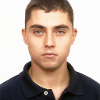
\includegraphics{ist173891}
            \caption*{
                ist173891 --- David Gonçalves\par
                david.s.goncalves@tecnico.ulisboa.pt
            }
        \end{subfigure}%
        \begin{subfigure}{.5\textwidth}
        \centering
        \captionsetup{justification=centering}
            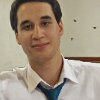
\includegraphics{ist194104}
            \caption*{
                ist194104 --- Leonardo Troeira\par
                leonardo.troeira@tecnico.ulisboa.pt
            }
        \end{subfigure}\vspace{6ex}
        
        \begin{subfigure}{1\textwidth}
        \centering
        \captionsetup{justification=centering}
            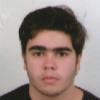
\includegraphics{ist194122}
            \caption*{
                ist194122 --- Francisco do Carmo\par
                francisco.baptista.carmo@tecnico.ulisboa.pt
            }
        \end{subfigure}
    \end{figure}
\end{titlepage}
    
%------------------------------------------------------------

\newpage

\section{Problem}
    
Password-based authentication has the advantage of being simple and convenient to use. However, there are too many attacks that can be performed remotely that render this authentication mechanism not secure enough on its own---phishing, XSS, SQLI, rainbow tables, dictionary attacks, brute force... to name a few.\par

As such, if we're seeking stronger security mechanisms, one option is to make use of multi-factor authentication, usually involving knowledge and possession. This poses a trade-off between security and usability however, since the user will be needing to carry something with him all the time (e.g. smartphone).\par

Besides authentication mechanisms, we're also faced with the challenge of data possibly being stolen, either by sniffing network packets or acquiring control over the victim's file system, among other possible attacks. Therefore, assuring that data is stored and transmitted securely (relying on encryption algorithms) is a must. And again, for additional security, we should have another factor of authentication.\par

\subsection{Requirements}

\begin{enumerate}
  \item The web server must have mechanisms to prevent XSS and SQLI.
  \item Communication between client and server must be done through a custom secure channel.
  \item The system must provide two-factor authentication.
  \item User files must be stored encrypted.
  \item User files must be decrypted only if the user has their smartphone nearby the client application.
  \item Communication with the server may only happen whilst the user has their smartphone nearby the client application.
  \item The system must provide fault tolerance. If the system crashes after decrypting the files, make sure that the files are not stored encrypted.
  \item Communication between the smartphone and client application must be done using a secure protocol.
  
\end{enumerate}


%------------------------------------------------------------

\newpage

\subsection{Trust assumptions}

Our problem assumes that the network and user's device (e.g. PC) cannot be trusted. However, we assume that the user's device is not compromised while the user is using the app, and that the smartphone and server are not compromised either. We also assume that the server's certificate is trusted.

\section{Proposed solution}

For our solution, we shall create a simple website, separating the client logic (JavaScript) from the server logic (PHP). There will be a register and login forms, for which we shall sanitize user input and make use of SQL parameters in order to prevent XSS and SQLI respectively. The user's password shall be relatively secure (min. 10 chars, contain lowercase, uppercase, digits and symbols) and shall be stored hashed and salted in order to prevent it from being easily obtained by potential attackers, should the server's database be compromised. As an additional security layer for authentication, we shall use 2FA with the help of Duo SDK, thus leveraging the smartphone's proximity to the user as part of an increased security solution.\par

The user shall be able to download files from the website, encrypted with a new random symmetric key. We shall make a simple Android app that will generate the user's long-term RSA key pair at its installation and will store it in the user's smartphone. The smartphone and user's device shall connect through Wi-Fi, utilizing a secure protocol (e.g. WPA2/3). For extra security, the user's private key should be symmetrically encrypted with a password, which should be different than the user's login password (e.g. KeyStore). The symmetric key used to encrypt each file shall also be stored in the smartphone encrypted with the user's public key.\par

Our client application (website's JS) shall be able to view these encrypted files that were downloaded from the server (for simplicity we'll consider only txt files). In order for the client application to decrypt these files, the smartphone must be connected to the user's device. The system shall be fault tolerant---as soon as this connection is lost, the client application shall clean its state, thus the user shall no longer be able to view the encrypted files nor communicate with the server. We plan on using a stream cipher for encrypting / decrypting, as in theory we can have large files that don't fit in volatile memory. For binary fails the alternative would be decrypting to the disk and encrypting when proximity is lost, but this does not prevent other kinds of faults (e.g. PC shutdown).\par

For registration and login, a shared AES key shall be obtained using a secure protocol, we propose Diffie-Hellman. Subsequent communication between the user and the server shall be done using symmetric encryption with this key, in order to guarantee confidentiality. For integrity, a MIC can be generated using Galois/Counter Mode (GCM) mode. Our only authenticity guarantees are that either the client or server created the message. We could provide non-repudiation by signing the message and having freshness, but we'll not consider this for this project. DH provides us with perfect forward secrecy as long as we generate new key pair values every session, but it is susceptible to man-in-the-middle, so we shall sign the exchanged public values with long-term RSA private keys.\par

%------------------------------------------------------------

\setcounter{figure}{0} % Reset figure counter
\begin{figure}[H]
\centering
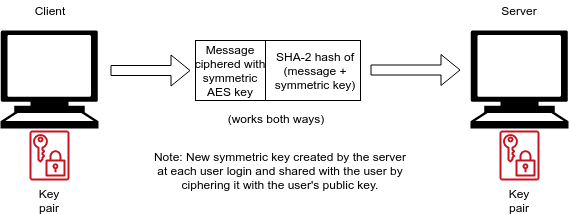
\includegraphics[width=11.8cm]{secure_channel.png}
\caption{Secure communication}
\end{figure}

%------------------------------------------------------------
\newpage
\section{Results}

\begin{itemize}

 \item \textbf{XSS and SQLi:} 
  To mitigate cross-site scripting we sanitize all the inputs that are not 100\% controlled by us (user inputs, server messages and smartphone messages) that end up being displayed. These validations are deployed both in the client side (JavaScript) and in the server side (PHP).

  To avoid SQL injections we used prepared statements to ensure that the values passed from the client to the server are compiled before being executed, thus not affecting the database in an undesirable way.
  
  \item \textbf{2FA:} 
  We decided to use Duo SDK, because it is a user-centric zero-trust security platform that allows an application to protect sensitive data. 
  
  In our approach the 2FA mechanisms are: "something the user has" (phone) and "something the user knows" (password).
  
  We managed to integrate Duo in our application successfully, making the user authenticate in the application only upon inserting the correct password and successfully respond to the Duo's challenge.
  
  \item \textbf{Proximity:}
  We assure that the user can only view, download or upload files (be logged in the system) when he is close to the computer that he is logged in. For this matter, the machine where the user is operating and the smartphone require to be connected in the same network. If connection with the smartphone is broken, proximity fails and the client is logged out, moreover losing access to the keys to decrypt the files.
  
  \item \textbf{WPA2:}
  We assume that the client and the smartphone are connected through WiFi under the WPA2 or WPA3 protocols. Making the connection between these two secure. In our project we simulated a smartphone using a virtual machine so when testing we did not use WPA2 for the communication.

  \item \textbf{Password strength:} 
  When creating a new account the user needs to enter a password that must be composed by at least 10 characters, and contain at least a lowercase, an uppercase, a digit and a symbol. By doing this we prevent brute-force attacks, and also by requiring this complexity we can mitigate common dictionary attacks. The users' passwords are stored in the server's database hashed and salted.

  \item \textbf{OSI layer:} We deal with the application, presentation and session layers which allow us to have some confidentiality in regard to the content of the messages and authentication. Still, we are unable to provide confidentiality in terms of knowing that a communication is going on and which resources are involved. For that a more in-depth protocol (e.g. Tunneling) would be required.
  
  \item \textbf{JS crypto issues:} We don't encrypt things on the client, and use the smartphone instead. One reason for this is the lack of JavaScript crypto libraries. The bonus is that it leverages proximity. The downside is that it is harder to program.
  
  \item \textbf{AES GCM:} Using AES operating in Galois/Counter Mode (GCM), we have a Galois Message Authentication Code (GMAC) that grants message integrity, so we can prevent bit-flip attacks on the payload.
  
  This approach is also useful because with GMAC we do not need create our own MACs or sign the messages' hashes. GMAC can only be generated by either the client or the server and that ensures some authenticity, however it does not ensure non-repudiation, for that we would need to sign the messages' hashes and implement freshness.

  \item \textbf{Diffie-Hellman:} 
  
  We made use of DH protocol for establishing a shared secret (at login and register) in order to have perfect forward secrecy. P and G values are always the same because they take a long time to generate and are not relevant for PFS, there are even standard values for these. However, private and public values are different each session. Because DH is susceptible to man-in-the-middle, we sign the public values with long-term RSA private keys. Except on the client's public value at register because the server has no way to verify the public value. Because we use Java and PHP we had to convert PEM to DER formats and vice-versa.
\end{itemize}

\section{Evaluation}
\begin{itemize}
    \item\textbf{Brute force:}
    Requiring a lengthy password with a wide range of possible characters mitigates brute force, for now, yet is inconvenient for the user and may no longer be sufficient in the future as computational power evolves. A better approach would be to limit the number of login attempts within a time period.

    \item \textbf{Duo registration:}
    Currently the user's smartphone is associated with Duo on the first login. It should be done at registration to avoid an attacker hijacking the account by potentially finding the user's server login password and associating his own smartphone with the account, should the attacker make the first login.

    However, because inserting the user in our database could possibly fail (e.g. mysql down) after associating the user's device with Duo, this would require deleting the user's account at Duo's Admin panel. For this, we'd need to use a PHP third-party library for making REST requests to the Duo's API and integrate it with our Duo account. This would give us some work to implement and is not the most important security fault of this project, so we chose to focus on other aspects considering the time we had available.

    \item \textbf{Check server's certificate:} We do not check if the server's certificate is valid as this would require a trusted 3rd-party. This is of course an essential step for a real world application.
    
    \item \textbf{Confidentiality:}
    It is possible to know that a communication is going on and with that information the attacker can try to infer what kind of message is being passed in the channel at that moment, and with more communications listened the attacker can start to observe a pattern that can lead to discover what kind of message we are sending. Since we use a stream cipher the length of the ciphertext is the same as the plaintext. Moreover, everyone can know what kind of resource the user is accessing in a time period (e.g. login.php, register.php, files.php)
    
    \item \textbf{Non-repudiation:}
    Our solution does not implement non-repudiation nor logging. It is also possible to perform replay attacks within a session as we do not have freshness implemented.
    
    \item \textbf{Encrypting files + Fault tolerance:}
    We were unable to implement file encryption / decryption in time. But we implemented .txt viewing in our client app and proximity detection, which would be the building block for file decryption fault tolerance.
    
    \item \textbf{Android app:}
    We decided to implement a Desktop app to make the implementation of this project easier considering the time we had available. But in a real world scenario we'd have to port our Java app do Android, which shouldn't be too difficult.
    
\end{itemize}

\section{References}

\begin{itemize}
  \item \textbf{Duo SDK:} Duo's trusted access solution is a user-centric zero-trust security platform to protect access to sensitive data at scale for all users, all devices and all applications.\par https://duo.com/product/every-application/supported-applications/apis\par
  Found: Yes\par
  Installed: No\par
  Tested: No\par
\end{itemize}

\end{document}